\documentclass[12pt,a4paper]{article}
\usepackage[margin=2cm]{geometry}
\usepackage{xeCJK}
\usepackage{fontspec}
\setCJKmainfont{Noto Serif CJK TC}[Script=CJK]
\usepackage{amsmath,amssymb}
\usepackage{graphicx}
\usepackage{fancyhdr}
\setlength{\headheight}{14.5pt}
\addtolength{\topmargin}{-2.5pt}
\usepackage{hyperref}
\usepackage{listings}
\usepackage{enumitem}
\usepackage{titlesec}
\usepackage{caption}
\usepackage{indentfirst}
\usepackage{booktabs}
\usepackage{longtable}
\usepackage{multirow}
\usepackage{array}
\usepackage{tabularx}
\usepackage{float}
\usepackage{minted}
\setlength{\parindent}{2em}
\pagestyle{fancy}
\fancyhf{}
\cfoot{\thepage}
\linespread{1.3}
\setminted{
    linenos,                % 行號
    frame=lines,            % 上下框線
    framesep=5pt,           % 程式碼與邊框距離
    numbersep=8pt,          % 行號與程式碼距離
    fontsize=\scriptsize,   % 字體大小
    breaklines,             % 自動換行
    tabsize=4,              % tab 寬度
    rulecolor=\color{black},% 框線顏色
    xleftmargin=1.5em       % 左側縮排
}

\title{生醫光電導論期末作業}
\author{B12508026戴偉璿}
\date{\today}

\begin{document}

\maketitle

\lhead{生醫光電導論期末作業}
\rhead{B12508026戴偉璿}

\begin{enumerate}
  	\item 昂貴的顯微鏡的鏡頭使用高級多層鍍膜光學玻璃，能消除色差、像差；廉價的顯微鏡則是使用壓克力或單片樹脂，邊緣易模糊、產生色散。此外，昂貴的顯微鏡的照明系統可能採用模組化Koehler照明，光線極度均勻且可精密調節；廉價的顯微鏡則是LED 簡易直射，光線不均勻，容易反光或產生暗角。這導致昂貴的顯微鏡有更好的放大倍率、解析度。
  	\item 在電子顯微術中，可成像體積反比於解析度的三次方，這代表解析度美提昇一倍，所需要的資料量就增加八倍，導致「大體積神經重建」與「原子級結構解析」在單一技術下幾乎不可能同時實現。 關於三種電子顯微鏡：
  	\begin{itemize}
    	\item SEM是三者中體積覆蓋能力最強的技術。它透過電子束掃描樣品表面並逐層削掉重建，可以處理立方毫米等級的組織體積，解析度大約5-20 nm。這個解析度足以辨識神經元的軸突、樹突與突觸小泡的整體輪廓，卻無法看見蛋白質的內部構象。對於大體積神經網路的三維重建而言，SEM 提供了是整個神經迴路的外觀，告訴我們哪些神經元彼此相連、突觸分布在哪裡。
    	\item TEM居中，電子束穿透超薄切片成像，解析度可達 1-5 nm，成像體積約在立方微米等級。搭配electron tomography，可以重建小範圍內的三維結構，清晰呈現突觸緻密帶與突觸後膜的整體形態。然而，傳統 TEM 需要化學固定與重金屬染色，可能在樣品中造成人工假象，也無法達到解析蛋白質原子結構所需的精度。整體而言，TEM承接了 SEM 建立的宏觀輪廓，將視野縮小到單一突觸的層級。
    	\item cryo-EM是解析度最高的技術。樣品在玻璃化冷凍狀態下保留幾乎天然的分子構象，完全避開化學固定的偽影。透過冷凍電子斷層掃描搭配子斷層圖平均，在原位細胞環境中將重複出現的蛋白複合物疊加平均，將解析度提升至0.3-0.5 nm，此解析度足以看見蛋白質的二級結構。若再結合單顆粒分析，甚至可達 0.12  nm的近原子解析度。但他的樣品厚度必須 <500 nm，龐大的組織體積無法直接處理。
  	\end{itemize}
	這三個尺度的資料要無縫連接，關鍵在於建立一套共同的座標系統，也就是所謂的correlative microscopy。實驗流程從 SEM 開始，在毫米尺度建立神經迴路的全局地圖，從中挑選具代表性的目標突觸。接著透過螢光標記與光學顯微鏡（CLEM）精確定位目標區域，再以聚焦離子束將該區域減薄為冷凍薄片，進入 cryo-ET 的成像流程，在微米尺度確認突觸形態與蛋白複合物的原位位置。最後對反覆出現的複合物做子斷層圖平均，達到奈米至次奈米的結構解析，並將得到的原子模型重新對應回最初 SEM 建立的神經迴路座標中。

	如此一來，每個尺度的資料都共享同一套座標變換，使得「某條神經迴路中某個突觸的某個蛋白複合物處於何種構象狀態」這個橫跨多個數量級的問題，得以被完整且連貫地回答。三種技術的價值不在於競爭，而在於各自不可替代地填補了物理上無法被其他技術覆蓋的尺度區間。
	\item 近紅外線（650-950 nm）之所以常用於測量大腦活動，是因為這個波段恰好落在「生物光學窗口」（如圖~\ref{fig:window}），血紅素和水對它的吸收都很低，光可以穿透頭皮與顱骨抵達腦皮質。此外，氧合與去氧血紅素在這個波段有不同的吸收特性，因此可以藉由偵測光強度變化來推算局部血氧濃度的變化，進而反映神經活動。
	
	傳統的Beer-Lambert law假設光在均勻透明介質中沿直線傳播，光程長度已知且固定，這在澄清溶液中完全成立；但生物內部組織複雜，充滿細胞膜、蛋白質等微結構，光進入後會被強烈散射而無法直線傳播，實際光程遠大於理想距離，導致傳統定律嚴重低估濃度。修正後的Beer-Lambert law為此引入了一個差分光程因子（Differential Pathlength Factor）來補償散射造成的路徑加長，並改為只計算吸光度的變化量而非絕對值。如此，可消除難以量化的靜態散射背景，從而估算出血氧濃度的相對變化。
	\begin{figure}[H]
		\centering
		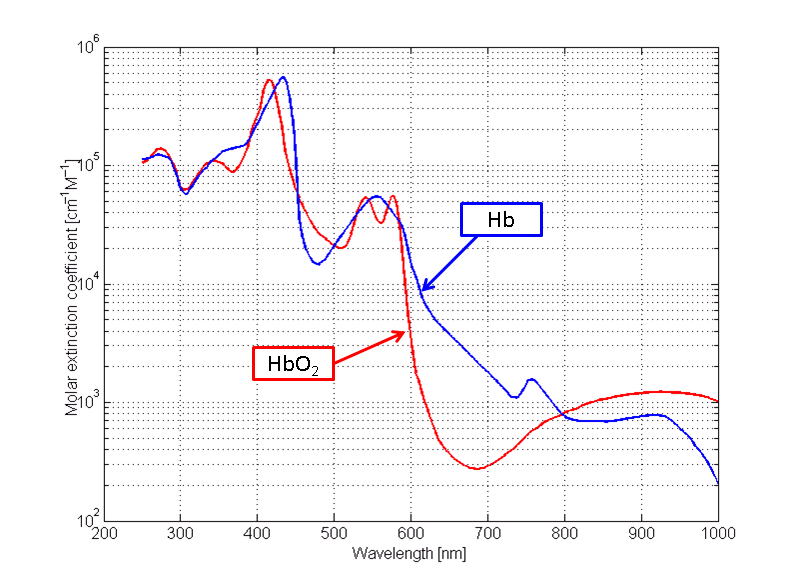
\includegraphics[width=0.8\textwidth]{src/window.png}
		\caption{生物光學窗口示意圖，近紅外線波段（650-950 nm）位於吸收最低的區域。圖片來源：維基百科}
		\label{fig:window}
	\end{figure}
	\newpage
	\item 共聚焦顯微鏡（圖~\ref{fig:confocal}）的光源、樣品焦平面、偵測器前的針孔，三者被設計在光學上共享同一個焦點，這種幾何關係使其能夠從厚標本中切出一個薄薄的光學截面。
	
	傳統螢光顯微鏡的問題在於：當你聚焦在某一層時，上下其他層的螢光分子也會被激發，這些焦平面以外的光會模糊地疊加在影像上，使整張影像不清楚且缺乏層次感。共聚焦顯微鏡在偵測器前放置一個極小的針孔（pinhole），控制聚焦的位置以解決此問題。
	
	雷射光經過聚光鏡後被聚焦成一個點光源，照射在樣品的特定焦平面上。來自這個焦平面的螢光訊號沿原路返回後，會被精確地聚焦在針孔所在的位置，順利通過針孔抵達偵測器。然而，來自焦平面上方或下方的離焦光，雖然同樣被收集進物鏡，但它們返回後無法聚焦在針孔的同一位置。這些光在針孔平面上呈現的是一個模糊的大光斑，大部分被針孔的邊緣擋掉，幾乎無法通過。
	
	針孔的大小直接決定了光學切片的厚度（亦即軸向解析度）。針孔越小，被擋掉的離焦光越多，光學切片越薄，但同時通過的訊號光也越少，影像會變暗；針孔越大則反之，切片厚度增加，但訊號亮度提升。因此針孔大小是一個需要根據實驗需求權衡的參數，在實務上通常設定在一個Airy disk大小左右以平衡解析度與訊號強度。

	成像切片的距離則由物鏡的焦距與數值孔徑決定。高數值孔徑的物鏡可以收集更大角度的光，使焦點更加集中、景深更淺，搭配小針孔後可以獲得非常薄的光學切片，約 0.5-1 $\mu$m。透過步進馬達沿 Z 軸逐層移動焦平面，每次只記錄當前焦平面的清晰訊號，最後將一系列的二維截面疊加重建，便得到整個厚標本的三維影像。這就是共聚焦顯微鏡能夠對厚標本進行光學切片的本質原因，它利用了針孔的空間濾波效果，在光學上隔絕了來自其他深度的雜訊。
	\begin{figure}[H]
		\centering
		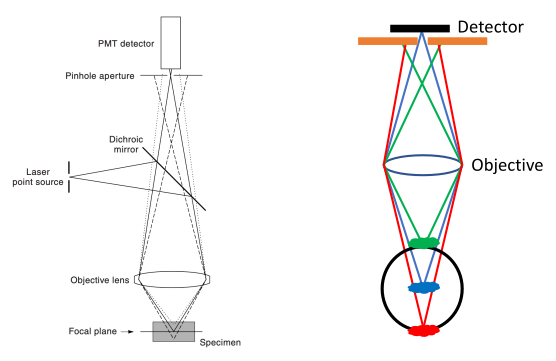
\includegraphics[width=0.8\textwidth]{src/confocal.png}
		\caption{共聚焦顯微鏡的光路示意圖，針孔位置決定了只有焦平面上的光能通過。圖片來源：朱麗安老師上課簡報}
		\label{fig:confocal}
	\end{figure}
	\item 傅立葉域OCT的兩種主要實作方式分別是光譜域OCT（Spectral-Domain OCT, SD-OCT）與掃頻光源OCT（Swept-Source OCT, SS-OCT）。
	
	SD-OCT 使用寬頻光源同時照射樣品，在偵測端以光柵將返回的干涉光依波長分散，再用 CCD 或 CMOS 同時記錄所有波長的干涉光譜。由於所有深度的資訊都被編碼在這一條光譜中，只需對其做傅立葉轉換便能重建出完整的深度剖面，不需要像時域 OCT 一樣機械式地掃描，因此速度大幅提升。

	SS-OCT 則是使用一個波長隨時間快速掃描的可調諧雷射作為光源，在時間軸上依序發出不同波長的光，搭配單點的平衡偵測器記錄每個瞬間的干涉訊號。掃完一個完整波長範圍後，同樣對時間序列做傅立葉轉換重建深度資訊。由於使用同調長度更長的雷射光源，SS-OCT 可以達到更深的成像深度，在波長選擇上也更靈活，例如使用 1300 nm 波段以減少組織散射，適合眼前節或血管等較深層結構的成像。

	\item 在課堂上學到的所有超解析度影像技術中，我對於Structured Illumination Microscopy（SIM）最感興趣。SIM 的原理是利用一組已知空間頻率的條紋光照射樣品，這些條紋光與樣品中細微結構的空間頻率相互作用，產生莫爾條紋。這些莫爾條紋包含了原本超出光學顯微鏡解析極限的高頻訊息。透過多角度、多相位的條紋照明，收集多組影像後進行數學重建，就能將這些高頻訊息解碼出來，實現約兩倍於傳統顯微鏡的解析度提升。這種顯微鏡沒有使用什麼高深的元件，利用了一般人家裡紗窗就能看見的效果，實現了超解析度的成像，非常的巧妙。

\end{enumerate}

\end{document}